\documentclass[10pt,a4paper]{article}
\usepackage[latin1]{inputenc}
\usepackage[pdftex]{graphicx}
\usepackage{amsmath}
\usepackage{amsfonts}
\usepackage{amssymb}
\usepackage{pseudocode}

\title{Advanced HUD Indicator (v2)}
\author{John [Moggie100] Vidler}
\begin{document}
\maketitle

\tableofcontents

\section{Overview}
The Advanced HUD Indicator (Adv. HUD) was designed to allow users to draw directly onto the screen and aid in the creation of dynamic graphic displays primerily for vehicles.

While version 1 acheived this to a small degree, with the precreated graphical elements allowing developers to draw certain types of graphics with ease, freedom was limited to targetting displays and some minor system's status displays without requiring far more scripted entites (SENTs) than is convenient.

Since the development of the Expression Gate and the further development of Egate2 and the in-game editor by Syranide, it has been proven that high-speed parsing of human readable script is possible in Garrys Mod (GMod) Lua, and as such, it would a far better development to use a similar scripting approach to the HUD.

\section{Language Selection}
Unfortunately, the languages with already implemented parsers in Lua are unusable for the task of drawing on-screen elements without extreme modification or complex in-game scripting.  Therefore it is nessicary to use a more appropriate language for \textit{markup} of HUD elements.

I highlight \textit{markup} in the previous sentence as important as this problem has already largely been solved.  HTML has been shown to be popular and easy to understand as a language for defining elements on a screen.  However, some of the concepts of web scripting languages do not transfer as well as others for HUD usage, text-flow for one is less useful in a HUD scripting language as developers may want to have text overlaying images, but will want text to be kept inside block areas.

A simpler way to create a managable script would be to use a less complex and established markup form.  Enter XML.

\subsection{XML - The Extensible Markup Language}

XML is \textit{ideal} for this class of problem, as it easily allows for the definition of nested blocks while allowing functionality to be extended without breaking the overall language definition, giving great freedom in the way of variables and tag names.

This freedom is the main reason for choosing XML as the language base for my markup language, however other advantages are also present, such as ease of use, as most developers have used XML in some form at one point or another, allowing them to quite easily slip in to using the markup here.

\section{HML - HUD Markup Language}

Obviously, XML in its raw form is not ready to be used as a full HUD scripting language, so additional tags and variables need to be defined.

However, before this can be concreted the final form of the markup must be defined, otherwise it could lead to issues later on when non-standard parameters break the schema becuase they were not considered at the start.

Consider the simple case of a small blue semitransparent box being centered in the screen; 

\begin{verbatim}
<rectangle x=CENTER-10 y=CENTER-10 width=20 height=20 color=(0,0,255,100) />
\end{verbatim}

In this simple case we have already used singletons, global variables, evaluations and vectors, giving a good point to start off the creation of a symbol set.

Tokenizing the script is relitavely simple, producing an output of...

\begin{quote}
LBRACE, NAME, PARAMNAME, EQ, GLOBAL, NEG, LITERAL, PARAMNAME, EQ, GLOBAL, NEG, LITERAL, PARAMNAME, EQ, LITERAL, PARAMNAME, EQ, LITERAL, PARAMNAME, EQ, VECSTART, LITERAL, COMMA, LITERAL, COMMA, LITERAL, COMMA, LITERAL, VECEND, SLBRACE
\end{quote}

...which shows one form of EVALUATE, three forms of PARAMETER, three forms of VALUE one form of VECTOR, and one form of TAG... All of which is described in the HML BNF section.

\section{Realtime Editing}

The parser offers no real delay in processing for clientside operations, and would cause no lag for multiplay as all of the code can be ran on the clients.

This allows almost real-time drawing of the user scripts as they are editing, giving direct feedback.  The one snag is that rendering at the HUD layer causes the components to draw behind the editor window, obscuring tham somewhat, and drawing after the HUD layer would obscure the editor.  Ergo; an additional buttons could be added to show an `n' second preview of the script.

However, as soon as any variables are used in the script, the value becomes unknown at the preview stage, so rendering during a preview would not really be viable.  Therefore, in all cases where render behavior cannot be defined, the component should be hidden, and the user notified.

\section{Input Lookup and Insersion}

Inputs prove a particular problem for rendering, as the values cannot simply be referenced and updated, as the render table is clientside and the lookup table is serverside.  Additionally, simply invoking the server to return a value to a given client for each lookup is impractical, as even for one simple variable the network traffic would be immense, calling the server one or more times per tick!

To solve this, I will implement the following:

\subsection{Server}

Run parser, generate lookup index and set default values.

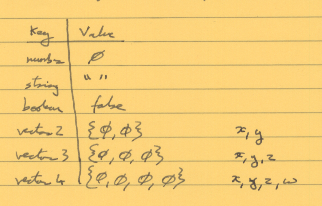
\includegraphics[scale=0.75]{images/server_lookup_table_types.png}

When an input is fired, it is looked up in the table, and sets the appropriate value.  This value is then sent to the client which performs the same lookup as the server, and the renders to the HUD.

\subsection{Client}

When a variable of type $"input_*"$ is seen, the code should check its variable table for the variable name, then use the value associated.  This is an identical operation to constant insersion, except performed at runtime on the client, rather than at parse time on the server.

\subsubsection{Example Table Requiring Lookup Operations}

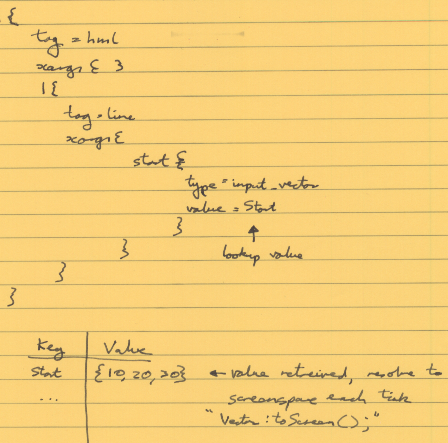
\includegraphics[scale=0.75]{images/parse_table_with_input_and_lookup_table.png}

\section{Additional Tags and Extensibility}

The alternative to presets is to increase the tag-name set by including the old indicators among the new tag lists.  This would bot help to keep the symbol set clean, and at the same time increase the `richness' of the language (HML 1.0).

However, by adding these elements to the main core of HML, the cleanliness of the language is compromised, leading to far more complex code to generate graphics on the screen.

Parhaps to combat this, an approach similar to E2 would be employed; whereby tag render functions are added to lookup tables, rather than being hard coded, then as requests for new tags come in they can simply add themselves to the table and be automaticly included in the render phase.

For this approach to be safe, however, the core functionality for HML should be kept seperate from the custom lookup table, otherwise core operations (lines, rectangles, and so forth) could become corrupted by malicious or useless code causing render artifacts to manifest on client's screens.

Unfortunately, this cannot be easily avoided on the custom lookup table, as there is no real way to seperate malicious code from valid.

The core commands, however, can be protected by either not allowing the table to be changed (method overrides) or by keeping a checksum and rejecting the table if it fails testing.

The simplest method for lookups would be to use the tag name sa the key, and have a render function as the value, then, during the validation phase, the parser can look up any tag name, displaying a warning if none is found.

\subsection{Backwards Compatability}

In the previous version, each indicator type was defined as a group of discrete elements, reducing the overall freedom for the user, but allowing fairly impresside HUDs for very little network lag.

The issue of network latency has been largely removed in version 2, as most of the information for displaying screen elements is sent at the 'compilation' stage, and only values are sent from inputs when they change, or when a HUD is hooked by a player.  (In the case of a hook, the entire table is sent as a 'glon' object to refresh the client's local table)

Elements missing data (unsent values on hook) are merely skipped until the next tick.

One option for feedback for this would be to show a loading-style progress bar as data is transferred at roughly the center of the screen, in a way much akin to the Advanced Duplicator's 'ghosting' and 'pasting' progress indicators.


\subsection{Presets}

As for the indicators using in version 1, they could be defined as a 'preset', and loaded in as a pseudo-include, this allowing user-made presets.

However, this does mean that the minimal data required to normally send these indicators would be increases (dependant on the complexity of the indicator itself) and the overall complexity of HML would increase to cope eith preset syntax (additional parameters, more complex loading, inline include, special HML fragments, unloadable on their own -no context- and so forth.)


\section{Dynamic Values in HML}

Updates are pushed to the clients;

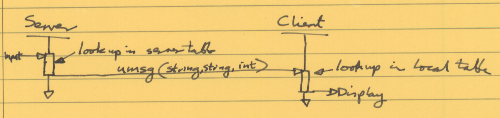
\includegraphics[scale=0.75]{images/push_updates.png}

At the serverside, the input lookup table is as follows;

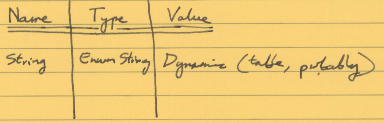
\includegraphics[scale=0.75]{images/serverside_lookup_table.png}

Where the values are stored as an appropriate representation of their type, ergo;

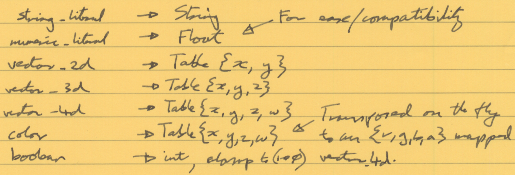
\includegraphics[scale=0.75]{images/serverside_lookup_types.png}

The precise type of the update "umsg" will depend on its update type. By selecting the type first, the content can be dynamicly parsed as required.  The general "umsg" format is therefore;

	$umsg \rightarrow \left[ \left( String \right) input\_name \right] \left[ \left( Integer \right) input\_type \right] \left[ Payload \rightsquigarrow \right] $

Where "Payload" is defined as the following;

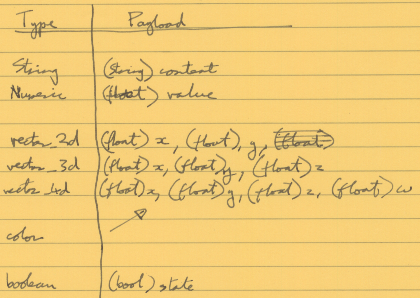
\includegraphics[scale=0.75]{images/payload_data_desc.png}

NOTE:  Booleans are defined as \textit{true} for \textit{any other value} than \textbf{zero}, and default to false.

\subsection{Macros}

When a variable is expected, but the renderer reads one of the following constants; LEFT, RIGHT, CENTRE, TOP, BOTTOM; the values are calculated from the tag-parent's context, and are defined as follows:

\begin{tabular}{|l|l|}
\hline Constant & Definition \\ 
\hline CENTRE & The mathematical centre of the parent, can be a value, or a vector2; \\
& $ = \left\lbrace 50\%,50\% \right\rbrace  $ vector2 form \\
& $ = 50\% $ value form \\ 
\hline LEFT & The extreme left-hand-side of the shape in a conventional layout, \\ 
& or in the case of a Derma entity, the left-hand border + 'n' pixels \\ 
& for spacing. \\
& $ = 0\% $ \\ 
\hline RIGHT & The extreme right-hand-side of the parent, see LEFT. \\
& $ = 100\% $ \\
\hline TOP,BOTTOM & The top-most, or bottom-most edge of the parent, see LEFT. \\
& $ = 0\%, 100\% $ \\
\hline 
\end{tabular} 

\section{Complex Shape Interface}

Because of the high number of values to describe complex, poly-point shapes would require a large number of I/O lines, memory based access is preferable, as it compresses an entities entire input set into one line.

Additionally, this would allow E2 and CPU access to HUD elements using readCell(), writeCell() and generic IO for the CPU, also giving the possibility for custom macros to access values via an E2 extension.

However, this does mean that mapped memory should follow a very strict schema, otherwise user confusion could occur.

Vectors should have the form; $(x,y(,z(,w)))$, colours; $(r,g,b(,a))$ conceptually, but should be stored as follows;

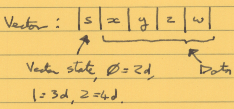
\includegraphics[scale=0.75]{images/memory/vector_format.png}

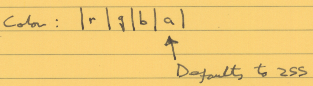
\includegraphics[scale=0.75]{images/memory/color_format.png}

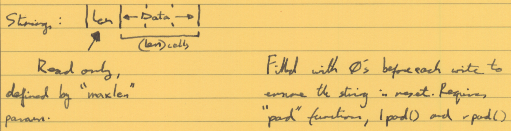
\includegraphics[scale=0.75]{images/memory/string_format.png}

By employing a length char, we can keep the memory clean, at the expense of slight user inconvenience, however, this does mean that (stupid) users can just set very high max lengths, causing the server to update very slowly - so to combat this, a server cvar will be created to set the upper limit for "maxlen" parameters.

\subsection{Naming}

Because memory access uses only one input, and the individual value names are meaningless here, the tag requires an additional parameter; "memory" such that a memory input name can me selected. Additonally, this parameter can be used to turn on/off memory I/O

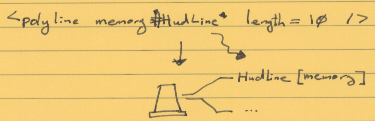
\includegraphics[scale=0.75]{images/memory/memory_input.png}

The length parameter in the above tag defines the number of points this polyline will have.  This parameter changes to 'sides' for a 'polygon' tag, but has the same effect.



\section{Quickref}
\subsection{HML Tags}

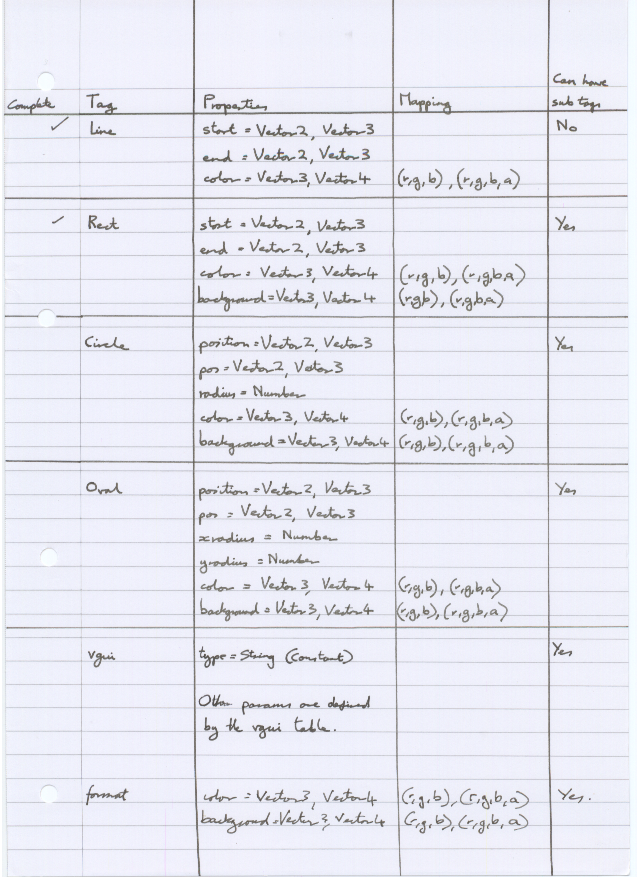
\includegraphics[scale=0.75]{images/quickref/tags.png}

\section{HML BNF}
This section details HML in BNF.  Some of the symbols (notibly 'GLOBAL') are context sensitive, and as such cannot easily be defined in BNF, therefore, for these symbols, I have expressed their function in "{}" blocks.

\subsection{Special Symbols}
These symbols are not really part of any definitions, but are important as they help define particular input strings more easily.

\begin{quote}
NULL		= ""\linebreak
HASH		= "\#"
\end{quote}

\subsection{Separators}
Seperators break up the input into nice processable chunks.

\begin{quote}
COMMA		= ","\linebreak
SPACE		= " "
\end{quote}

\subsection{Math Symbols}
Mathematical symbols, allowing calculations to be performed in inline expressions within tags.

Useful for positioning code, as statements such as \textit{x=CENTER-10} give functionality that would not otherwise be possible, locking UIs into the top left hand corner of all users displays.

Additionally, the expressions can be used to scale the graphical symbols to each user's screen resolution.

\begin{quote}
EQ = "="\linebreak
NEG	= "-"\linebreak
PLUS = "+"\linebreak
TIMES = "*"\linebreak
DIVIDE = "/"
\end{quote}

\subsection{Block Construction}
Start and end marker tokens for tags to construct blocks.

\begin{quote}
LBRACE		= "<"\linebreak
RBRACE		= ">"\linebreak
SLBRACE		= "</"\linebreak
SRBRACE		= "/>"\linebreak
LBRACKET	= "("\linebreak
RBRACKET	= ")"
\end{quote}

\subsection{Identifiers}

\begin{quote}
LABEL		= CHARSEQUENCE
\end{quote}

There is an additional \textit{GLOBAL} however, this is context specific, but basicly a list of known character sequences to check for and replace with a variable. useful for obvious constants like "CENTER", "WIDTH", "HEIGHT" and so forth.

\subsection{Special Variable Types}

\begin{quote}
VECTOR = LBRACKET VALUE COMMA VALUE COMMA VALUE RBRACKET\linebreak
COLOR = LBRACKET VALUE COMMA VALUE COMMA VALUE RBRACKET | LBRACKET VALUE COMMA VALUE COMMA VALUE COMMA VALUE RBRACKET\linebreak
INPUT = HASH CHARSEQUENCE
\end{quote}

\subsection{Parameters}

\begin{quote}
PARAMLIST	= NULL | PARAM | PARAM PARAMLIST\linebreak
PARAM		= LABEL EQ EXPRESSION\linebreak
VALUE		= LITERAL | VARIABLE | VECTOR\linebreak
CHARSEQUENCE	= CHAR | CHAR CHARSEQUENCE\linebreak
STRING		= QUOTE CHARSEQUENCE QUOTE\linebreak
LITERAL		= NUMERIC | STRING
\end{quote}

\subsection{Tags}
\begin{quote}
OPENTAG		= LBRACE LABEL PARAMLIST RBRACE\linebreak
CLOSETAG	= SLBRACE LABEL RBRACE\linebreak
SINGLETAG	= LBRACE LABEL PARAMLIST SRBRACE\linebreak
BLOCKLIST	= BLOCK | BLOCK BLOCKLIST\linebreak
BLOCK		= OPENTAG CLOSETAG | OPENTAG BLOCK
\end{quote}

\subsection{Expressions}
It should be noted here that expressions should follow BODMAS convention such that they are easily understandable by most people.

\begin{quote}
EXPRESSION	= VALUE | VALUE OPERATOR VALUE | EXPRESSION OPERATOR EXPRESSION | LBRACKET EXPRESSION RBRACKET\linebreak
OPERATOR	= NEG | PLUS | TIMES | DIVIDE
\end{quote}

\subsection{Example First Pass Tokenization}

The following input string;
\begin{verbatim}
<rectangle x=CENTER-10-#XOFFSET y=CENTER-10-#YOFFSET width=20 height=20 color=(0,0,255,100) />
\end{verbatim}

Becomes;

\begin{verbatim}
[LBRACE] [LABEL]
[LABEL] [EQ] [GLOBAL] [NEG] [LITERAL] [NEG] [HASH] [CHARSEQUENCE]
[LABEL] [EQ] [GLOBAL] [NEG] [LITERAL] [NEG] [HASH] [CHARSEQUENCE]
[LABEL] [EQ] [LITERAL]
[LABEL] [EQ] [LITERAL]
[LABEL] [EQ]
[LBRACKET]
	[LITERAL] [COMMA]
	[LITERAL] [COMMA]
	[LITERAL] [COMMA]
	[LITERAL]
[RBRACKET] [SLBRACE]
\end{verbatim}

(Separated by sub-block, where space == newline)

\end{document}